\chapter{OpenCL}
\label{h:opencl} 
OpenCL is een framework voor het uitvoeren van parallelle berekeningen. Deze berekeningen kunnen uitgevoerd worden op \'e\'en of meerdere gewone processoren (CPU) of op \'e\'en of meerdere grafische kaarten. Een CPU of een GPU noemen we een apparaat (device). We zullen het OpenCL-jargon niet vertalen naar het Nederlands om verwarring te vermijden.

\section{Het model}
In dit hoofdstuk beschrijven we de voornaamste OpenCL-concepten. Deze zijn onafhankelijk van het apparaat en zelfs van het soort apparaat.
\subsection{Verdeling van het werk}
\subsubsection{Work-items}
Een reeks instructies die we parallel kunnen uitvoeren noemen we een kernel. De eenheid van werk dat door een kernel verwerkt wordt noemen we een work-item. Het apparaat voert de kernel, in parallel, uit op de work-items. Een work-item komt dus overeen met \'e\'en thread. Het aantal work-items is meestal afhankelijk van de invoer van het algoritme.

Neem als voorbeeld het optellen van twee vectoren. $\vect{c} = \vect{a} + \vect{b}$. We kunnen dit op een seri\"ele manier berekenen:

\begin{lstlisting}
void sum(const double a[], const double b[],
        double c[], int N)
{
    for(int index = 0; index < N; index++)
    {
        c[index] = a[index] + b[index];
    }
}
\end{lstlisting}
We kunnen dit herschrijven naar:
\begin{lstlisting}
void sum(const double a[], const double b[], double c[], int N)
{
    for(int index = 0; index < N; index++)
    {
        inner(a, b, c, index);
    }
}
void inner(const double a[], const double b[], double c[],
    const int index)
{
    c[index] = a[index] + b[index];
}
\end{lstlisting}
%In welke volgorde we de index kiezen maakt eigenlijk niets uit.
We kunnen deze berekening dus makkelijk in parallel berekenen.
Een OpenCL-kernel uit een programma die dezelfde berekening doet kan er als volgt uitzien:
\begin{lstlisting}
__kernel void innerKernel(__global const double a[],
    __global const double b[], __global double c[])
{
    int i = get_global_id(0);
    c[i] = a[i] + b[i];
}
\end{lstlisting}
Het eerste dat opvalt is dat er een paar sleutelwoorden zoals \code{\_\_kernel} en \code{\_\_global} zijn bij gekomen. \code{\_\_kernel} geeft aan dat de functie een kernel is die gelanceerd kan worden. \code{\_\_global} geeft aan dat het om globaal geheugen gaat. (Zie \ref{h:opencl:geheugen})

Wat echter veel belangrijker is, is dat de parameter \code{N} verdwenen is. Waar we vroeger \code{inner} \code{N} keren na elkaar uitvoerden, gaan we nu \code{innerKernel} %\code{N} keer
in parallel uitvoeren. Er zijn \code{N} work-items. 

In dit voorbeeld komt \'e\'en element uit de vector overeen met \'e\'en work-item, maar dit moet niet altijd zo zijn. We gebruiken \code{get\_global\_id(0)} om te achterhalen welk work-item we verwerken.

\subsubsection{NDRange}
In het bovenstaande voorbeeld associ\"eren we met een work-item een nummer. Het eerste work-item krijgt nummer nul, de tweede nummer \'e\'en enzovoorts. Het is ook mogelijk om met elk work-item een 2-tupel te associ\"eren. Dit kan bijvoorbeeld nuttig zijn als we matrices willen optellen. We kunnen dan een work-item met een element van de matrix associ\"eren. Het eerste element van de tupel komt dan overeen met de rij van de matrix en de tweede met de kolom. OpenCL laat zelfs 3-tupels toe, maar geen 4-tupels.

We zeggen dat het volledige werk overeen komt met de NDRange en dat de NDRange verdeeld wordt in work-items. Wanneer we een kernel lanceren, geven we mee hoe groot de NDRange is. Of met andere woorden, hoeveel work-items er zijn. NDRange staat voor N dimensionele Range. Wanneer we een gewoon getal associ\"eren met een work-item spreken we over een 1DRange. Wanneer we 2-tupels gebruiken spreken we over een 2DRange en bij 3-tupels over een 3DRange. Een 3DRange heeft drie dimensies: X, Y en Z.

\subsubsection{Work-groups}
OpenCL verplicht ons om de NDRange op te delen in groepen. Zo \'e\'en groep noemen we een work-group. Waarom we deze groepen moeten maken zullen we later zien. Wanneer de NDRange bestaat uit n-tupels dan is de grootte van een work-group ook een n-tupel.

De X-component van de work-groupgrootte moet een gehele deler zijn van de X-component van de grootte van de NDRange. Hetzelfde geldt ook voor de Y -en de Z-component. Dit betekent dat het aantal work-items in de NDRange een geheel veelvoud is van het aantal work-items in een work-group. AMD beperkt de grootte van de work-groups tot maximaal 256 work-items. Een work-group met grootte (8, 8, 8) heeft in totaal 512 work-items en is dus te groot.


\begin{figure}[]
\centering
\includegraphics{workitem}
\caption{\label{workitem}Een visualisatie van work-items, wavefronten, work-items en de NDRange. Bron: handleiding AMD\cite[p.~1-9]{amd}.}
\end{figure}

\subsection{Geheugen}
\label{h:opencl:geheugen}
OpenCL kent drie soorten geheugen:
\begin{itemize}
    \item Privaat geheugen: enkel toegankelijk binnen work-item.
    \item Lokaal geheugen: gedeeld met alle work-items in binnen een work-group, niet toegankelijk buiten de work-group.
    \item Globaal geheugen: toegankelijk voor alle work-items.
\end{itemize}

Gegevens in het RAM-geheugen kunnen enkel gekopi\"eerd worden naar het globaal geheugen. Een work-item kan dan de gegevens lezen uit het globaal geheugen en opslaan in het privaat geheugen. Work-items kunnen ook gegevens schrijven naar het lokaal geheugen. Deze gegevens kunnen dan door andere work-items binnen dezelfde work-group gelezen worden. Zie figuur \ref{geheugenCL} voor een schematische voorstelling van de gegevensstromen tussen de soorten geheugens.

\begin{figure}[]
\centering
\includegraphics[scale=0.5]{geheugenCL}
\caption{\label{geheugenCL}Een schematische overzicht van de gegevensstromen tussen de soorten geheugens.}
\end{figure}

\subsection{Synchronisatie}
Niet alle work-items lopen synchroon. Dit kan voor problemen zorgen wanneer een work-item gegevens moet lezen die door een ander work-item geschreven zijn. Daarom is het mogelijk om synchronizatiepunten toe te voegen. Dit kan op twee niveau's. We kunnen alle work-items in een work-group synchroniseren en alle work-items in de NDRange. Wanneer een work-item een synchronizatiepunt tegen komt zal het daar stoppen met uitvoeren tot alle andere work-items stil staan aan het synchronizatiepunt. Dit heeft meestal een negatief effect op de performantie en moet zo veel mogelijk vermeden worden.

%\section{<stuff over cpu en gpu>}

\section{Architectuur AMD Radeon HD 6970}
\subsection{Rekeneenheden}

Wanneer we een kernel lanceren gaat de GPU de work-groups verdelen over de compute-units. Dit is de taak van de Ultra-Threaded Dispatch Processor (UTDP). De UTDP zal pas nieuwe work-groups toewijzen wanneer de compute-unit tijdelijk geen werk meer heeft.  Wanneer een work-group toegewezen is zeggen we dat de work-group actief is.

\label{WGvolg}
De UTDP zal work-groups in de volgende volgorde activeren. Eerst wordt work-group (0, 0, 0) geactiveerd. Daarna is work-group (1, 0, 0) aan de beurt. Wanneer de UTDP door X-waarden is geroteerd, is het de beurt aan work-item (0, 1, 0). We noemen dit een rij-eerst volgorde.

Elke compute-unit (CU) heeft een command-processor die verantwoordelijk is voor het selecteren en ophalen van de instructies. Omdat elke CU een eigen command-processor heeft, werken CU's volledig zelfstandig en los van alle andere CU's.

De compute-unit bestaat, naast de command-processor, ook uit 16 processing-elementen (PE). Alle processing-elementen binnen een compute-unit worden aangestuurd door de command-processor in de compute-unit. Hierdoor voeren alle processing-elementen altijd dezelfde instructie uit.

Een processing-element is ook gekend onder de naam stream core (SC). Een ALU wordt in de documentatie soms ook processing element genoemd. In deze tekst zullen we altijd de termen gebruiken zoals ze in bovenstaande paragraaf beschreven zijn.

De instructies zijn 128 bits lang en bestaan eigenlijk uit vier 32-bit instructies. Een 128-bit instructie noemen we een very long instruction word (VILW). Een processing-element bestaat uit vier ALU's die elk een 32-bit instructie uitvoeren. Sommige instructies zijn te zwaar om met \'e\'en ALU uit te voeren. Daarom kunnen twee of vier ALU's samengenomen worden om de zware instructie uit te voeren. Wanneer we een instructie uitvoeren duurt het acht cycli voor het resultaat ervan beschikbaar is voor een volgende berekening.

Zie figuur \ref{alu} voor een schematische voorstelling van de rekeneenheden.

\begin{figure}[h]
\centering
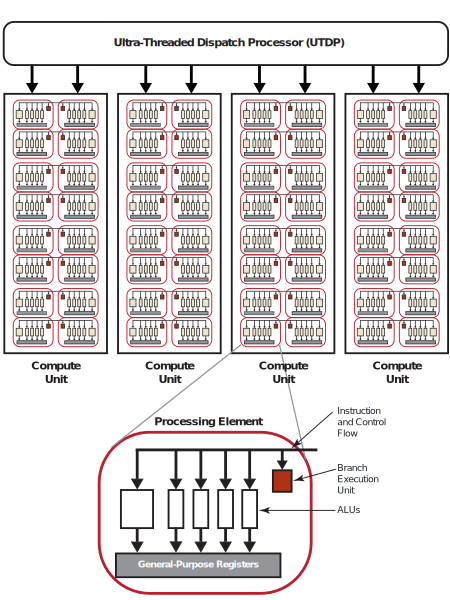
\includegraphics{alu}
\caption{\label{alu}Een schematische overzicht van de rekeneenheden. Bron: handleiding AMD\cite[p.~1-5]{amd}.}
\end{figure}

%\todo{Wavefront en relatie met work-items (misschien mapping hardware <-> workitems een apart hfdstk}


%\todo{tekening uit slide/handleiding}
%\todo{Ultra-Threaded Dispatch Processor}
%\todo{latency van 8 cycli}

\subsection{Wavefronten}
\label{wavefront}
Alle processing-elementen van de compute-unit voeren dezelfde instructie vier keer na elkaar uit. Elke cyclus voert een processing-element de instructie uit op een ander work-item. In de eerste cyclus voert het eerste processing-element het eerste work-item uit en het tweede processing-element het tweede work-item. De volgende cyclus voert het eerste processing-element het 17de work-item uit enzovoorts. Vier cycli maal 16 processing-elementen vormt een groep van 64 work-items. Zo een groep noemen we een wavefront. De vier cycli waarin dezelfde instructie wordt uitgevoerd noemen we een golf. De 16 processing-elementen die gelijktijdig worden uitgevoerd noemt men een kwart-wavefront.

Alle work-items van een wavefront komen uit dezelfde work-group. We splitsen de work-group op in groepjes van 64 work-items. Als het aantal work-items in een work-group geen geheel veelvoud is van 64, zal het laatste groepje aangevuld worden met 'lege' work-items. Wanneer we een work-group activeren, activeren we eigenlijk de wavefronten.

Merk op dat alle workitems in het wavefront tijdens golf dezelfde instructie uitvoeren. Hieruit volgt dat alle work-items in een wavefront altijd synchroon lopen.



\subsection{Geheugen}

\subsubsection{Lokaal geheugen}
Elke compute-unit heeft 32KiB lokaal geheugen. Dit geheugen wordt gedeeld door alle actieve work-groups op de compute-unit. Het is voor een work-group echter niet mogelijk om te communiceren met een andere work-group via dit lokaal geheugen. Het lokaal geheugen bestaat uit 32 banken die elk vier bytes breed zijn. Dit betekent dat de eerste vier bytes naar de eerste bank gaan, de volgende vier naar de tweede enzovoorts. De 129ste byte gaat terug naar de eerste bank. ($4 \times 32 = 128$)

Elk processing-element kan elke cyclus twee vierbyte aanvragen doen. Deze twee adressen moeten niet aaneensluitend zijn. Elke cyclus kan elke bank \'e\'en aanvraag behandelen. Indien de 32 $(2 \times 16)$ vierbyte aanvragen allemaal naar verschillende bank gaan, kan men in theorie snelheden tot 2,7 TB/s over de hele GPU halen. Wanneer verschillende aanvragen gelijktijdig naar dezelfde bank gaan, worden de aanvragen geserialiseerd. We spreken dan van een bankconflict. De compute-unit blijft dan dezelfde wavefront uitvoeren tot elke aanvraag behandeld is. In elke cyclus zal \'e\'en aanvraag behandeld worden.

\subsubsection{Registers}
Elke compute-unit heeft 16Ki registers van elk vier keer vier bytes. Dit geeft in totaal 256KiB en is dus acht keer zo groot als het lokaal geheugen. De registers worden gedeeld door alle actieve work-groups op de compute-unit maar de work-items hebben enkel toegang tot de registers die aan hen zijn toegewezen. Elke cyclus kan elk processing-element twaalf vierbytes lezen uit het registergeheugen. Dit is juist genoeg om elke ALU een multiply-add in enkele precisie te laten uitvoeren in \'e\'en cyclus.

\subsubsection{Globaal geheugen}
De GPU heeft 2GiB geheugen waarvan we 1GiB als globaal gedeeld geheugen kunnen gebruiken. Dit geheugen wordt gedeeld door alle work-items over het hele apparaat. Wanneer een wavefront een geheugenaanvraag doet, zal de compute-unit dit bundelen en doorsturen naar \'e\'en van de acht geheugencontrollers. Elke controller is op zijn beurt verbonden met meerdere banken. We zeggen de geheugencontroller de gegevens verwerken die naar \'e\'en kanaal gaan. Er is \'e\'en geheugencontroller per kanaal.

De controller verwerkt de aanvraag en 300 tot 600 cycli later is het resultaat beschikbaar. Dit betekent echter niet dat de geheugencontroller 300 tot 600 cycli stil staat. Er kan \'e\'en 128 bit aanvraag gedaan worden per geheugencyclus. Tijdens de 300 tot 600 cycli wordt de wavefront in een wachttoestand gezet en de compute-unit voert een ander wavefront uit. Het wavefront wordt pas terug actief wanneer alle geheugenaanvragen van alle work-items volledig rond zijn.

Net als bij het lokaal geheugen bepaalt het adres naar welk kanaal de aanvraag gaat. De eerste 256 bytes gaan naar het eerste kanaal en naar de eerste bank van dat kanaal, de volgende 256 gaan naar het tweede kanaal en diens eerste bank enzovoorts. De 2049ste byte gaat terug naar het eerste kanaal, maar dan in de tweede bank. Wanneer we door alle banken geroteerd zijn zal de volgende byte terug naar de eerste bank van het eerste kanaal gaan. Het aantal banken is niet gedocumenteerd.

Het kan gebeuren dat meerdere work-item hetzelfde kanaal en/of dezelfde bank aanspreken. Wanneer dit gebeurt zullen de aanvragen geserialiseerd worden. Dit gebeurt zowel voor lees -als schrijfoperaties. We spreken zowel bij banken als bij kanalen over kanaalconflicten. We doen dit om het contrast met bankconflicten in het lokaal geheugen te bewaren.

%\todo{Mooie tekeningen}



\subsubsection{Constant globaal geheugen, L1 -en L2 caches}
Omdat het globaal geheugen een lage bandbreedte en een hoge traagheid heeft, zijn er enkele caches ingebouwd. Elke compute-unit heeft een L1-cache en elk kanaal heeft een L2-cache. De programmeur heeft echter geen rechtstreekse controle over deze caches, maar men kan wel een betere performantie verkrijgen als men er wel rekening mee houdt. Caching wordt enkel toegepast in twee gevallen:
\begin{itemize}
    \item Bij een aanvraag dat gaat naar geheugen dat nooit verandert. Dit om inconsistenties te voorkomen.
    \item Wanneer alle work-items van een wavefront in dezelfde cyclus hetzelfde adres uitlezen.
\end{itemize} 

Wanneer het adres al bij het compilen bekend is en de inhoud niet van waarde verandert, dan wordt de inhoud gecached in de constanten-cache. Deze inhoud wordt automatisch ingeladen vlak voor het gebruik ervan en levert snelheden tot 256 bytes per cyclus per compute-unit. Dit is twee maal zo snel als het lokaal geheugen en maar drie maal zo traag als de registers. Dit komt meestal voor bij eenvoudige constanten en kernel-parameter.

Zie figuur \ref{geheugen6970} voor een schematische voorstelling van het globaal geheugen en alle caches.

\begin{figure}
\centering
\includegraphics{geheugen6970}
\caption{\label{geheugen6970}Een schematische voorstelling van het globaal geheugen met de caches en Fast -en CompletePath. Bron: handleiding AMD\cite[p.~6-2]{amd}.}
\end{figure}

\subsubsection{Vergelijking soorten geheugen}
De verschillende soorten geheugen hebben verschillende groottes en snelheden. We verwijzen naar tabel \ref{geheugenSnelheden} voor een overzicht hiervan.

\begin{table}
	\centering
    \begin{tabular}{|l |c| r |r|}
		\hline
        Geheugen 	& \'e\'en per 		&
        \begin{tabular}{@{}c@{}}Snelheid \footnote{over hele GPU} \\ (KiB)\end{tabular} &
        \begin{tabular}{@{}c@{}}Grootte \footnote{over hele GPU}\\	(TB/s)\end{tabular}  \\
        \hline
        Register	& compute-unit		& 6144		& 16,220 \\
        Lokaal		& compute-unit		& 768		& 2,703 \\
        Constant	&vier compute-units	& 48		& 5,407 \\
        L1-cache	& compute-units		& 192		& 1,352 \\
        L2-cache	&geheugencontroller	& 512		& 0,451 \\
        Globaal		& apparaat			& 1GiB		& 0,176 \\
        \hline
    \end{tabular}
    \caption{\label{geheugenSnelheden}Een vergelijking van de soorten geheugen in de GPU. Bron: handleiding AMD\cite[p.~D-3]{amd}}
\end{table}

\section{Aandachtspunten voor optimalisaties}
\subsection{Wavefronten}
Men kan er best voor zorgen dat het aantal work-items in een work-group een geheel veelvoud is van 64. Wanneer dit niet het geval is, zullen wavefronten aangevuld worden met 'lege' work-items. Hierdoor zal de rekenkracht beperkt worden. Stel dat er maar 32 work-items in een work-group zitten. Er zullen dan maar twee van de vier cycli gebruikt worden voor nuttig rekenwerk. De rest van de tijd zal er niets gebeuren. Hierdoor zal de rekenkracht van de GPU halveren.

Het is ook belangrijk om voldoende wavefronten actief te hebben om alle vormen van traagheid te maskeren. Vanaf dat er genoeg wavefronten actief zijn, heeft het geen zin meer om er meer actief te maken. Er zijn echter enkele limieten op het aantal wavefronten die gelijktijdig actief kunnen zijn. Indien er niet genoeg wavefronten zijn zullen zowel de compute-unit als de geheugencontroller stil vallen.

\subsubsection{Traagheid maskeren}
Wanneer we een instructie uitvoeren duurt het acht cycli voor het resultaat ervan beschikbaar is. Een wavefront bestaat uit vier cycli, dus twee wavefronten per compute-unit volstaan om deze traagheid te maskeren.

Een globaal geheugenaanvraag duurt 300 tot 600 cycli. Laten we voor deze berekening 400 cycli nemen en stellen dat er na elke leesinstructie, vijf rekeninstructies zijn en dan terug een leesinstructie enzovoorts. Een wavefront bestaat uit vier cycli die elk vijf instructies uitvoeren voor ze zelf een geheugenaanvraag doen. Er zijn voor dit voorbeeld dus 20 (400 / (4 * 5)) wavefronten per compute-unit nodig om de traagheid van het globaal geheugen te maskeren.

\subsubsection{Limieten}
De eerste en meest eenvoudige limiet is dat er maximaal 512 wavefronten tegelijkertijd actief kunnen zijn. Dit zijn er ongeveer 21 per compute-unit en dus net genoeg voor het bovenstaande voorbeeld.

De registers worden door alle work-items op een compute-unit gedeeld. Het aantal nodige registers per work-item is gekend na de compilatie. Stel dat elk work-item 32 registers nodig heeft. Dat zijn er 2Ki per wavefront. Er zijn 16 Ki registers beschikbaar, dus er kunnen dan exact acht wavefront gelijktijdig actief per compute-unit. In de handleiding van AMD \cite{amd} kan u tabel 6.8 terugvinden op p.~6-28. Deze tabel geeft een overzicht van het effect van het gebruik van het lokaal geheugen op het maximaal aantal actieve wavefronten.

Net als het aantal registers is ook het lokaal geheugen gedeeld en is de grootte beperkt. De hoeveelheid lokaal geheugen per work-group is gekend wanneer we de kernel lanceren. Stel dat een work-group uit 100 work-items bestaat en 4KiB lokaal geheugen nodig heeft. We hebben 32KiB lokaal geheugen, dus er kunnen acht work-groups gelijktijdig actief zijn op elke compute-unit. E\'en work-group komt overeen met twee wavefronten (64 < 100 < 128). Dit geeft dan 16 actieve wavefronten per compute-unit.  In de handleiding van AMD \cite{amd} op p.~6-26 bevindt zich geeft een tabel die een overzicht van de impact van het aantal gebruikte registers op het maximaal aantal actieve wavefronten.


\subsection{Globaal geheugen}
\subsubsection{Kanaalconflicten}
Wanneer er een kanaalconflict is zullen er compute-units stil vallen. Dit zal zeker een impact hebben op de performantie. Een eenvoudige methode om kanaalconflicten te vermijden is door aaneensluitende work-items en work-groups aanvragen te laten doen naar aaneensluitende geheugenplaatsen. Hierdoor zullen alle aanvragen gespreid worden over alle kanalen en banken. Work-groups zijn aaneensluitend als ze vlak na elkaar geactiveerd worden. Zie \ref{WGvolg} voor de volgorde waarin work-groups geactiveerd worden. 

\subsubsection{FastPath of CompletePath}
Er zijn twee manieren waarop geheugen opgevraagd kan worden, via FastPath en via CompletePath. FastPath kan enkel gegevens laden en opslaan. Deze gegevens moeten een veelvoud van 32 bits groot zijn. CompletePath kan ook gegevensstructuren verwerken die kleiner zijn dan 32 bit. Bijvoorbeeld bytes en short. CompletePath ondersteunt ook atomische operaties.

Deze extra functionaliteit komt echter met een grote kost. Empirische testen \cite[p.~6-3]{amd} hebben aangetoond dat CompletePath wel vier keer ze traag kan zijn. CompletePath moet dus zoveel mogelijk vermeden worden.

Zie figuur \ref{geheugen6970} voor een schematische overzicht van Fast -en CompletePath en de plaats ervan in het globaal geheugen.

\subsubsection{Float4 of float}
Het globaal geheugen stuurt gegevens in blokken van 128 bytes. Dit komt overeen met een float4 of een double2. In een empirische test wordt een buffer gekopi\"eerd. Eerst met behulp van float's en daarna met behulp van float4's. Uit de test blijkt dat de bandbreedte bij het kopi\"eren met float4's ongeveer een derde hoger is dan met float's. \cite[p.~6-11]{amd}

\subsection{Lokaal geheugen}
\subsubsection{Float4}
\label{fl4BankConfl}
Beschouw onderstaand fragment uit een kernel waarbij een work-group bestaat uit 64 work-items en de NDRange slechts \'e\'en dimensie heeft.
\begin{lstlisting}
    ...
    __local float4* l[64];
    float4 v;
    ...
    v = l[get_local_id(0)];
    ...
\end{lstlisting}
Het lokaal geheugen kan twee vierbyte waarden per cyclus verwerken, een float4 bestaat uit vier vierbyte waarden en een wavefront bestaat uit vier cycli. Men zou dus denken dat de geheugenaanvraag in totaal acht cycli in beslag zal nemen. Maar omdat we eerst de eerste twee vierbytes opslaan en dan pas de volgende twee, gebruiken we elke cyclus slechts de helft van de banken en zal het in totaal 16 cycli duren voor alle geheugenaanvragen volledig rond zijn. Dit eenvoudig patroon moet vermeden worden.

\subsubsection{Alternatieven}
Er zijn alternatieven voor het lokaal geheugen die zeker overwogen moeten worden. Een eerste alternatief is de L1-cache. De L1-cache is niet rechtstreek controleerbaar en kunnen we enkel gebruiken voor lees-operaties. Het is ook kleiner dan het lokaal geheugen. Maar het heeft ook voordelen. De L1-cache wordt gedeeld door alle actieve work-groups op de compute-unit en het wordt impliciet gebruikt waardoor er geen extra cycli verloren gaan. Daarnaast krijgt het lokaal geheugen het moeilijk wanneer de gegevenstypes groter zijn dan acht bytes. (zie hierboven \ref{fl4BankConfl}) Het lokaal geheugen is maar twee maal zo snel als de L1-cache, maar moet wel eerst gevuld worden.

Een tweede alternatief is het registergeheugen. Dit geheugen is niet gedeeld met de andere work-items waardoor er meerdere kopie\"en van de gegevens bestaan. Aan de andere kant is het registergeheugen acht keer zo groot en zes maal zo snel als het lokaal geheugen. Een ander nadeel van het registergeheugen is dat de indexen al tijdens het compilen vast moeten liggen. Net als het lokaal geheugen heeft de programmeur hier volledige controle over en moet het eerst ingeladen worden.

Het laatste alternatief is de contanten-cache. Net als de L1-cache wordt dit geheugen impliciet gebruikt en is het enkel toegankelijk voor leesoperaties. Een ander nadeel is dat de adressen gekend moeten zijn bij compilatie. Het is ook zeer beperkt in grootte. De grootste voordelen zijn dat het twee maal zo snel is als het lokaal geheugen, geen problemen heeft met gegeventype die groter zijn dan acht bytes en dat het niet ingeladen moet worden.